% lrc_filter_design_guidelines.tex
% Design guidelines for L, LC, LCL and L(RC) filters: grid side of an active front end and
% output side of inverters feeding induction and permanent-magnet synchronous motors.
% pwr-control template (AAA_template_latex_settings); numbers of the worked examples:
% lrc_filter_example.py (python3, numpy only)
% Compile: pdflatex lrc_filter_design_guidelines.tex  (twice, for references)
% Rev. 00 - October 2026 - first issue
\documentclass[10pt,a4paper]{scrartcl}
% ===================== PACKAGES =====================
\usepackage[british]{babel}
\usepackage[tmargin=1in, bmargin=1in, lmargin=0.75in, rmargin=0.75in]{geometry}
\usepackage[dvipsnames,table]{xcolor}  % prima di tikz, listings, ecc.

\usepackage{tikz}
\usepackage{graphicx}
\usepackage{pgfplots}
\pgfplotsset{width=12cm, compat=1.9}
\usepackage{setspace}
\usepackage{chemmacros}
\usepackage{chemfig}
\usepackage{esint}
\usepackage{tabularray}
\usepackage{makeidx}
\usepackage{epstopdf}
\usepackage{amssymb}
\usepackage{mathrsfs}
\usepackage{bm}
\usepackage{amsmath}
\usepackage{enumitem}
\usepackage[english]{varioref}
\usepackage{lipsum}
\usepackage{fancyhdr}
\usepackage{float}
\usepackage{empheq}
\usepackage[framemethod=tikz]{mdframed}
\numberwithin{equation}{section}
\usepackage{eso-pic}
\usepackage{calc}
\usepackage{nccmath}
\usepackage{caption}
\usepackage{subcaption}
\usepackage{gensymb}
\usepackage{amsfonts, amsthm, epsfig, epstopdf, titling, url, array}
\usepackage{tabularx}
\usepackage{makecell}
\usepackage{booktabs}
\usepackage{array}
\usepackage{siunitx}
\sisetup{input-digits=0123456789\pi}
\usepackage[symbol]{footmisc}
\usepackage{multicol}
\usepackage{boondox-cal}
\usepackage{blindtext}
\usepackage{changepage}
\usepackage{nomencl}
\usepackage{hyperref}
\usepackage{xurl}
\usepackage{ragged2e}
\usepackage[version=4]{mhchem}  % ← conflitto di opzioni
\usepackage{longtable}
\usepackage{chemformula}
\usetikzlibrary{arrows.meta,positioning,calc}

% ===================== SI UNITS =====================
\DeclareSIUnit\atm{atm}
\DeclareSIUnit{\var}{var}
\DeclareSIUnit{\pu}{p.u.}


% ===================== MATH OPERATORS =====================
\DeclareMathOperator{\rank}{rank}
\DeclareMathOperator{\atantwo}{atan2}
\DeclareMathOperator{\spn}{span}

% ===================== COMMANDS =====================
\newcommand{\abs}[1]{\left|#1\right|}
\newcommand{\sign}{\text{sign}}
\newcommand{\centered}[1]{\begin{tabular}{@{}l@{}} #1 \end{tabular}}

% ===================== COLORS =====================
\definecolor{mycolor1}{rgb}{0.97, 0.97, 0.97}
\definecolor{mycolor2}{rgb}{0.97, 0.97, 0.97}
\definecolor{tableShade}{gray}{0.9}

% ===================== THEOREM ENVIRONMENTS =====================
\theoremstyle{it}
\newtheorem{defn}{Definition}[section]
\newtheorem{assumption}{Assumption}[section]
\newtheorem{thm}{Theorem}[section]
\newtheorem{lemma}{Lemma}[section]
\newtheorem{corollary}{Corollary}[section]
\theoremstyle{definition}
\newtheorem{example}{Example}[section]

% ===================== CUSTOM ENVIRONMENTS =====================
\newenvironment{myitemize_1}{
	\begin{itemize}[topsep=0pt]
		\setlength{\topsep}{2pt}
		\setlength{\itemsep}{2pt}
		\setlength{\parskip}{2pt}
		\setlength{\parsep}{2pt}
	}{\end{itemize}}

\newmdenv[
innerlinewidth=0.5pt,
roundcorner=4pt,
backgroundcolor=mycolor2,
linecolor=mycolor1,
innerleftmargin=6pt,
innerrightmargin=6pt,
innertopmargin=6pt,
innerbottommargin=6pt
]{mybox}

% ===================== TABLE COLUMN TYPES =====================
\newcolumntype{Y}{>{\hsize=2\hsize}X}
\newcolumntype{Z}{>{\centering\arraybackslash\hsize=0.857\hsize}X}

% ===================== SECTION DEPTH =====================
\setcounter{secnumdepth}{3}
\setcounter{tocdepth}{3}

% ===================== PAGE STYLE =====================
\setlength{\headheight}{20pt}
\setlength{\headsep}{20pt}

\pagestyle{fancy}
\fancypagestyle{firstpage}{\rhead{}}
\fancyhead[L]{\slshape\nouppercase{\leftmark}}
\chead{}
\rhead{\includegraphics[height=0.75cm]{../../AAA_template_latex_settings/pwr-control_logo_doc.png}}
\lfoot{\href{http://www.pwr-control.com}{pwr-control.com}}
\cfoot{-\ \thepage\ -}
\rfoot{\textit{}}
\renewcommand{\headrulewidth}{0.4pt}
\renewcommand{\footrulewidth}{0.4pt}


\geometry{
	a4paper,
	top    = 2.5cm,
	bottom = 3.0cm,
	left   = 2.5cm,
	right  = 2.5cm
}

\hypersetup{
	colorlinks = true,
	urlcolor   = blue,
	linkcolor  = black,
	citecolor  = black
}

\pagenumbering{gobble}
% the document sits three levels below the repository root: logo path of settings.tex corrected here
\rhead{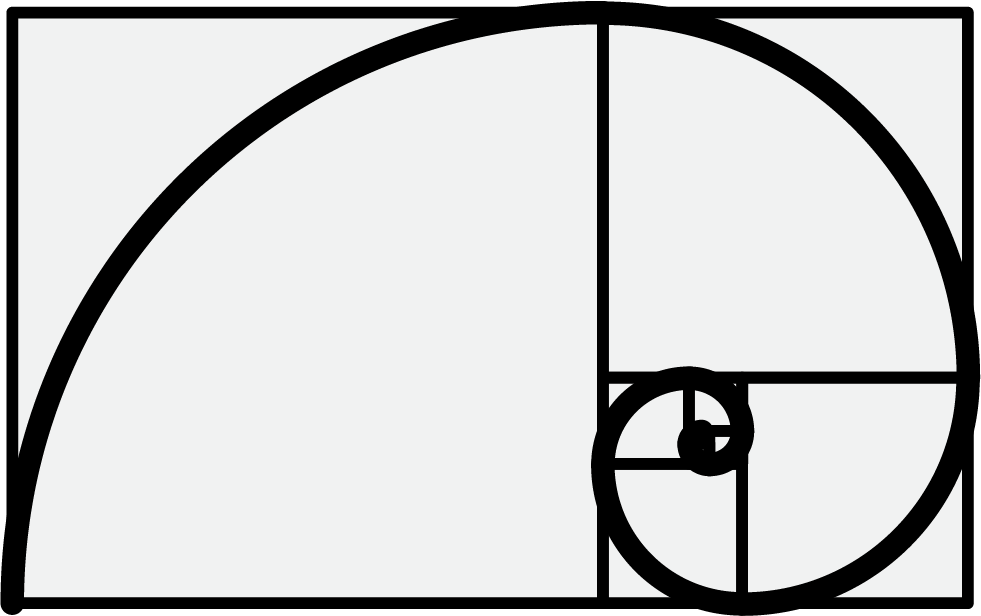
\includegraphics[height=0.75cm]{../../../AAA_template_latex_settings/pwr-control_logo_doc.png}}
\rfoot{\small Rev.~00}
\geometry{left=2.0cm, right=2.0cm}
\usepackage[european]{circuitikz}
\ctikzset{bipoles/length=0.9cm}

\sisetup{per-mode=symbol,range-phrase={\text{--}},range-units=single}
\setlist{nosep}
\setlength{\parindent}{0pt}
\setlength{\parskip}{3pt}
\allowdisplaybreaks

% --- shorthand ---
\newcommand{\Vdc}{V_{dc}}
\newcommand{\fsw}{f_{sw}}
\newcommand{\wsw}{\omega_{sw}}
\newcommand{\fres}{f_{res}}
\newcommand{\wres}{\omega_{res}}
\newcommand{\Lhf}{L_{hf}}
\newcommand{\Rhf}{R_{hf}}
\newcommand{\Cf}{C_{f}}
\newcommand{\Lf}{L_{f}}
\newcommand{\Lg}{L_{g}}
\newcommand{\pp}{\mathrm{pp}}
\newcommand{\rt}[1]{\text{\small\color{blue!60!black} #1}}

% =============================================================
%  DOCUMENT DATA (title page: AAA_template_latex_settings/titlepage.tex)
% =============================================================
\newcommand{\DocCategory}{Technical Note}
\newcommand{\DocField}{Power Electronics and Control Systems}
\newcommand{\DocTitle}{%
	{\fontsize{20}{24}\selectfont\bfseries L(RC) Filter Design Guidelines} \\[16pt]
	{\fontsize{16}{20}\selectfont\bfseries Grid-side filters for active front ends and output filters for induction and permanent-magnet motor drives}
}
\newcommand{\DocSubtitle}{Topologies, sizing relations, resonance placement, damping and interaction with the current control}
\newcommand{\DocAuthor}{Davide Bagnara}
\newcommand{\DocRevision}{00}
\newcommand{\DocDate}{October 2026}
\newcommand{\DocAbstract}{%
Design guidelines for the passive filters of two-level voltage-source converters: the L, LC, LCL and L(RC)L filter between an active front end (AFE) and a grid of given impedance, and the LC or L(RC) output filter between an inverter and an induction motor (IM) or a permanent-magnet synchronous motor (PMSM). The note first settles the switching ripple of the converter-side inductor, with exact closed forms for sinusoidal, space-vector and discontinuous PWM, the mean and the rms ripple over the fundamental period, and a comparison with the usual $\Vdc/(8\fsw L)$ rule. It then gives, for the grid side, the sizing of the converter inductor, of the capacitor (reactive power), of the grid inductor (attenuation at the switching frequency against IEEE~519), the placement of the resonance with respect to the grid frequency, the switching frequency and the critical frequency $f_s/6$ of the digital current loop, the passive damping options (series resistor, R--C branch) with their losses, and the interaction with the grid impedance. For the motor side it covers the reflected-wave overvoltage with long cables, the $dv/dt$ and sine filter options, the resonance window, the loaded resonance set by the high-frequency inductance of the machine (transient inductance of the IM, $L_d$/$L_q$ of the PMSM), the damping, the capacitor current and voltage budget, and the consequences for the current control and for sensorless (observer-based) control. Two sizing paths with worked examples (\SI{400}{V}/\SI{250}{kVA} AFE; \SI{110}{kW} IM and PMSM drives) and a bibliography close the note; the numbers are reproduced by the companion Python script.
}
\newcommand{\RevisionHistory}{%
	00 & October 2026 & First issue. & \DocAuthor \\
}
\newcommand{\MetaLabelA}{Project Repository}
\newcommand{\MetaValueAUrl}{https://github.com/pwr-control/repositories-documentation.git}
\newcommand{\MetaValueALabel}{repositories-documentation.git}
\newcommand{\MetaLabelB}{Calculation}
\newcommand{\MetaValueB}{Python 3 / NumPy (\texttt{lrc\_filter\_example.py})}

\begin{document}
% =============================================================
%  pwr-control LaTeX template - FRONTESPIZIO
%
%  Da richiamare come prima istruzione dopo \begin{document}:
%      \input{../../AAA_template_latex_settings/titlepage}
%
%  Il documento deve definire prima di \begin{document}:
%      \DocCategory   categoria del documento
%      \DocField      area tecnica
%      \DocTitle      titolo (una o due righe)
%      \DocSubtitle   sottotitolo
%      \DocAuthor     autore/i, separati da virgola
%      \DocRevision   numero di revisione corrente (es. 00)
%      \DocDate       data della revisione corrente
%      \DocAbstract   abstract
%      \RevisionHistory  righe della tabella di revisione, nel formato
%                        Rev. & Date & Description & Authors \\
%      \MetaLabelA \MetaValueAUrl \MetaValueALabel
%      \MetaLabelB \MetaValueB
% =============================================================

\providecommand{\DocCategory}{Technical Research Report}
\providecommand{\DocField}{Power Electronics and Control Systems}
\providecommand{\DocSubtitle}{}
\providecommand{\DocRevision}{00}
\providecommand{\DocAbstract}{}
\providecommand{\RevisionHistory}{%
	\DocRevision & \DocDate & First issue. & \DocAuthor \\
}

\titlepage

% ---- Intestazione centrata ----
\begin{center}
	{\Large\scshape \DocCategory}\\[8pt]
	{\large\scshape \DocField}
\end{center}

\vspace{30pt plus 4pt minus 14pt}
\noindent\rule{\linewidth}{0.8pt}

% ---- Titolo ----
\begin{center}
	\DocTitle
\end{center}

\vspace{4pt}
\noindent\rule{\linewidth}{2.2pt}

% ---- Sottotitolo ----
\begin{center}
	\begin{onehalfspace}
		{\large\itshape \DocSubtitle}
	\end{onehalfspace}
\end{center}

% ---- Authors / Revision / Date ----
\vspace{30pt plus 4pt minus 14pt}

\noindent
\begin{minipage}[t]{0.46\linewidth}
	\raggedright
	\textbf{Authors:}\\[2pt]
	\DocAuthor
\end{minipage}%
\hfill
\begin{minipage}[t]{0.22\linewidth}
	\centering
	\textbf{Revision:}\\[2pt]
	\DocRevision
\end{minipage}%
\hfill
\begin{minipage}[t]{0.30\linewidth}
	\raggedleft
	\textbf{Date:}\\[2pt]
	\DocDate
\end{minipage}

\vspace{10pt}
\noindent\rule{\linewidth}{0.8pt}

% ---- Abstract ----
\vspace{24pt plus 4pt minus 12pt}

\begin{center}
	\begin{minipage}{0.88\linewidth}
		\footnotesize
		\begin{onehalfspace}
			\textbf{Abstract:} \DocAbstract
		\end{onehalfspace}
	\end{minipage}
\end{center}

\vfill

% ---- Revision history ----
\begin{center}
	\begin{minipage}{0.96\linewidth}
		\centering
		{\footnotesize\scshape Revision history}\\[6pt]
		{\footnotesize
			\begin{tabular}{@{}cl>{\raggedright\arraybackslash}p{0.36\linewidth}>{\raggedright\arraybackslash}p{0.28\linewidth}@{}}
				\toprule
				\textbf{Rev.} & \textbf{Date} & \textbf{Description} & \textbf{Authors} \\
				\midrule
				\RevisionHistory
				\bottomrule
			\end{tabular}}
	\end{minipage}
\end{center}

\vspace{18pt plus 4pt minus 10pt}

% ---- Metadati in fondo ----
\noindent
\begin{tabular}{@{} r @{\quad} l @{}}
	\textsc{\MetaLabelA:} & {\href{\MetaValueAUrl}{\MetaValueALabel}} \\[3pt]
	\textsc{\MetaLabelB:} & {\MetaValueB}       \\[3pt]
\end{tabular}

% =============================================================
%  Fine frontespizio
% =============================================================
\newpage
\pagenumbering{arabic}
\setcounter{page}{1}

\tableofcontents
\newpage

\section{Scope and notation}
Two-level three-phase voltage-source converter (VSC) \cite{mohan2003,holmes2003} with DC link $\Vdc$, switching frequency $\fsw$ ($\wsw = 2\pi\fsw$), double-edge regular-sampled PWM with sampling frequency $f_s = \fsw$ (single update) or $2\fsw$ (double update). Two applications are treated with the same formulas: the grid side of an active front end (AFE), Fig.~\ref{fig:circ}(a), and the output side of a motor inverter, Fig.~\ref{fig:circ}(b). All quantities are per phase of the star equivalent; $V$ is the RMS line-to-line voltage, $V_{ph} = V/\sqrt3$, $I_n$ the rated RMS phase current, $\hat I_n = \sqrt2 I_n$. The base impedance is $Z_b = V^2/S_n$, $L_b = Z_b/\omega_1$, $C_b = 1/(\omega_1 Z_b)$ with $\omega_1 = 2\pi f_1$ the fundamental (grid or motor) angular frequency. Formulas are quoted without derivation except where the derivation is short and not found in the references.

\begin{figure}[htb]
\centering
\begin{circuitikz}[scale=0.9, every node/.style={transform shape}]
% (a) grid side
\draw (0,0) to[sV, l=$v_1$] (0,2)
      to[L, l=$L_1$, i=$i_1$] (2.6,2)
      to[L, l=$L_2$, i=$i_2$] (5.2,2)
      to[L, l=$\Lg$] (7.4,2)
      to[sV, l=$v_g$] (7.4,0) -- (0,0);
\draw (2.6,2) to[R, l=$R_d$, dashed] (2.6,1.1) to[C, l=$\Cf$] (2.6,0);
\draw (3.9,2) to[C, l=$C_2$] (3.9,1.1) to[R, l=$R_2$] (3.9,0);
\node[anchor=north west] at (2.9,2.0) {\scriptsize $v_c$};
\node at (3.7,-0.6) {(a) grid side: L ($\Cf = 0$), LCL, L(RC)L};
% (b) motor side
\begin{scope}[xshift=9.2cm]
\draw (0,0) to[sV, l=$v_i$] (0,2)
      to[L, l=$\Lf$, i=$i_i$] (2.6,2)
      to[generic, l={cable $Z_0,\tau$}, i=$i_s$] (5.0,2)
      to[R, l=$\Rhf$] (6.4,2)
      to[L, l=$\Lhf$] (7.8,2)
      to[sV, l=$e$] (7.8,0) -- (0,0);
\draw (2.6,2) to[R, l=$R_d$, dashed] (2.6,1.1) to[C, l=$\Cf$] (2.6,0);
\draw (3.9,2) to[C, l=$C_2$] (3.9,1.1) to[R, l=$R_2$] (3.9,0);
\node at (3.9,-0.6) {(b) motor side: LC, L(RC); $\Lhf = \sigma L_s$ (IM), $L_d,L_q$ (PMSM)};
\end{scope}
\end{circuitikz}
\caption{Filter structures. The damping is either the series resistor $R_d$ (dashed) or the parallel branch $C_2$--$R_2$ (the ``RC'' of L(RC)); only one of the two is used.}
\label{fig:circ}
\end{figure}

\section{Switching ripple of the converter-side inductor}
\label{sec:ripple}
The converter-side inductor ($L_1$ or $\Lf$) is sized first from its switching ripple. With the capacitor node a stiff voltage at $\fsw$ (LCL, LC) or a stiff grid (plain L), the phase current ripple over one switching period $T_{sw} = 1/\fsw$ is piecewise linear with slopes $(v_{1,n} - v_{ref})/L$, where $v_{1,n}$ is the converter phase voltage with respect to the load neutral ($0$, $\pm\Vdc/3$, $\pm 2\Vdc/3$) and $v_{ref}$ the reference. Let $m = \hat V_{ref}/(\Vdc/2)$ be the modulation index ($m \le 1$ for sinusoidal PWM, $m \le 2/\sqrt3 = 1.155$ for space-vector or third-harmonic PWM). All ripple figures scale as
\begin{equation}
\Delta i = k\,\frac{\Vdc}{\fsw L},
\label{eq:kdef}
\end{equation}
and the coefficient $k$ depends on the modulator, on $m$ and on the position $\theta$ along the fundamental period. Two closed forms cover the two extremes (phase voltage at its peak, $\theta = 0$, and at its zero crossing, $\theta = 90^\circ$):
{\small
\begin{align}
k_{\pp}(\theta = 0) &= \frac{m}{4}\Big(1 - \frac{m}{2}\Big)\ \text{(SPWM)},\qquad
\frac{m}{4}\Big(1 - \frac{3m}{4}\Big)\ \text{(SVM, THI)},\qquad
\frac{m}{2}\Big(1 - \frac{3m}{4}\Big)\ \text{(DPWM, clamped phase)},
\label{eq:kpk}\\
k_{\pp}(\theta = 90^\circ) &= \frac{\sqrt3\,m}{12} = \frac{m}{6.93}\qquad \text{(all modulators)}.
\label{eq:kzc}
\end{align}}
Eq.~\eqref{eq:kpk} follows from $\Delta i_{\pp} = v_{ref}\,(T_0 + |T_{0a} - T_{0b}|)/(2L)$, with $T_0 = T_{0a} + T_{0b}$ the total zero-vector time and $T_{0a}$, $T_{0b}$ its split between $000$ and $111$ (equal for SVM, $(1-m)T_{sw}/2$ and $(1-m/2)T_{sw}/2$ for SPWM at $\theta = 0$, all on one vector for the clamped phase of DPWM); at $\theta = 0$, $T_0/T_{sw} = 1 - 3m/4$. Eq.~\eqref{eq:kzc} follows from the two active vectors of equal dwell $T_1 = T_2 = (\sqrt3/4)\,m\,T_{sw}$ giving $\pm\Vdc/3$ to the phase at its zero crossing. The peak-to-peak ripple is largest at the phase peak for small $m$ and at the zero crossing for large $m$ (crossover at $m = 0.56$ for SVM, $0.85$ for SPWM). The worst case over the whole linear range is therefore
\begin{align}
\Delta i_{\pp,max} &= \frac{\Vdc}{4\sqrt3\,\fsw L} = \frac{\Vdc}{6.93\,\fsw L} && \text{(SPWM, at } m = 1), \label{eq:worst}\\
\Delta i_{\pp,max} &= \frac{\Vdc}{6\,\fsw L} && \text{(SVM/THI, at } m = 2/\sqrt3\text{; DPWM, at } m = 2/3 \text{ and } 2/\sqrt3). \nonumber
\end{align}
The RMS value of the ripple over the fundamental period, needed for the inductor and capacitor losses and for the harmonic current injected into the capacitor, is given by the harmonic distortion factor of Holmes and Lipo \cite{holmes2003}:
\begin{equation}
I_{rip,rms} = \frac{\Vdc}{24\,\fsw L}\sqrt{\mathrm{HDF}(m)},\qquad
\mathrm{HDF} =
\begin{cases}
\tfrac32 m^2 - \tfrac{4\sqrt3}{\pi} m^3 + \tfrac98 m^4 & \text{(SPWM)},\\[4pt]
\tfrac32 m^2 - \tfrac{4\sqrt3}{\pi} m^3 + \Big(\tfrac{27}{16} - \tfrac{81\sqrt3}{64\pi}\Big) m^4 & \text{(SVM)}.
\end{cases}
\label{eq:hdf}
\end{equation}
Table~\ref{tab:ripple} lists $k$ for the maximum and the mean (over the fundamental period) peak-to-peak ripple and for the RMS ripple, computed exactly by the companion script; the closed forms \eqref{eq:kpk}--\eqref{eq:hdf} are reproduced to four digits.

\begin{table}[htb]
\centering\footnotesize
\caption{Ripple coefficient $k$ of \eqref{eq:kdef}, written as $1/x$: maximum peak-to-peak over the fundamental period, mean peak-to-peak, RMS of the ripple. Two-level VSC, double-edge regular sampling, isolated neutral.}
\label{tab:ripple}
\begin{tabular}{@{}c ccc ccc ccc@{}}
\toprule
 & \multicolumn{3}{c}{SPWM} & \multicolumn{3}{c}{SVM / THI} & \multicolumn{3}{c}{DPWM1 ($60^\circ$ clamping)} \\
\cmidrule(lr){2-4}\cmidrule(lr){5-7}\cmidrule(lr){8-10}
$m$ & max pp & mean pp & RMS & max pp & mean pp & RMS & max pp & mean pp & RMS \\
\midrule
0.4   & 1/12.5 & 1/17.6 & 1/67 & 1/14.3 & 1/18.7 & 1/68 & 1/7.1 & 1/10.4 & 1/35 \\
0.6   & 1/9.5  & 1/13.7 & 1/52 & 1/11.6 & 1/15.3 & 1/55 & 1/6.1 & 1/8.8  & 1/30 \\
0.8   & 1/8.3  & 1/12.1 & 1/44 & 1/8.7  & 1/14.4 & 1/49 & 1/6.3 & 1/8.9  & 1/31 \\
0.9   & 1/7.7  & 1/11.4 & 1/41 & 1/7.7  & 1/14.0 & 1/47 & 1/6.8 & 1/9.4  & 1/32 \\
1.0   & 1/6.9  & 1/10.9 & 1/37 & 1/6.9  & 1/13.5 & 1/45 & 1/6.9 & 1/10.4 & 1/35 \\
1.1   & --     & --     & --   & 1/6.3  & 1/13.0 & 1/42 & 1/6.3 & 1/11.5 & 1/37 \\
1.155 & --     & --     & --   & 1/6.0  & 1/12.8 & 1/40 & 1/6.0 & 1/11.9 & 1/38 \\
\bottomrule
\end{tabular}
\end{table}

\begin{mybox}
\textbf{Which ripple formula to use.} The widely used $L = \Vdc/(8\fsw\Delta i_{\pp})$ is neither the maximum nor the mean: at $m \approx 1$ with SVM the true maximum is $\Vdc/(6.9\fsw L)$ (\SI{15}{\percent} above the rule), the worst case over $m$ is $\Vdc/(6\fsw L)$ (\SI{33}{\percent} above, the value used by Liserre et al.~\cite{liserre2005} and Reznik et al.~\cite{reznik2014}), while the mean peak-to-peak over the fundamental is $\Vdc/(13.5\fsw L)$ (\SI{40}{\percent} below). The rule is a fair ``typical period'' estimate; it is not an upper bound. Recommended use: (i) size $L$ and check the saturation current $\hat I_n + \Delta i_{\pp,max}/2$ with the maximum of Table~\ref{tab:ripple} at the largest $m$ of the application ($\Vdc/(6\fsw L)$ when the converter reaches the hexagon, $\Vdc/(7\fsw L)$ for an AFE at $m \approx 1$); (ii) use the RMS column, or \eqref{eq:hdf}, for the capacitor current, the damping losses and the harmonic current at $\fsw$; (iii) with discontinuous PWM at the same $\fsw$ the ripple is up to twice that of SVM at low $m$, so compare at equal switching losses ($\fsw$ raised by $1.5$).
\end{mybox}

\section{Filter structures and transfer functions}
\label{sec:tf}
With $Z_1 = sL_1$, $Z_2 = s(L_2 + \Lg)$ and $Z_c$ the impedance of the shunt network of Fig.~\ref{fig:circ}(a), and the grid voltage a short at the switching harmonics,
\begin{equation}
\frac{i_1}{v_1} = \frac{Z_c + Z_2}{Z_1 Z_2 + Z_c (Z_1 + Z_2)},\qquad
\frac{i_2}{v_1} = \frac{Z_c}{Z_1 Z_2 + Z_c (Z_1 + Z_2)},\qquad
\frac{i_2}{i_1} = \frac{Z_c}{Z_c + Z_2}.
\label{eq:tf}
\end{equation}
For the undamped LCL ($Z_c = 1/(s\Cf)$), writing $L_2' = L_2 + \Lg$,
\begin{equation}
\frac{i_2}{v_1} = \frac{1}{s^3 L_1 L_2' \Cf + s(L_1 + L_2')},\qquad
\wres^2 = \frac{L_1 + L_2'}{L_1 L_2' \Cf},\qquad
\frac{i_2}{i_1} = \frac{1}{1 + s^2 L_2' \Cf},\qquad
\omega_2^2 = \frac{1}{L_2'\Cf}.
\label{eq:lcl}
\end{equation}
At the switching frequency the attenuation of the LCL with respect to its own converter current is
\begin{equation}
k_a = \left|\frac{i_2}{i_1}\right|_{\wsw} = \frac{1}{\wsw^2 L_2' \Cf - 1} \approx \Big(\frac{f_2}{\fsw}\Big)^2,
\qquad\text{equivalently \cite{liserre2005}}\quad
\frac{i_2(\wsw)}{i_{L}(\wsw)} = \frac{1}{\big|1 + r\,(1 - \wsw^2 L_1 \Cf)\big|},\ \ r = \frac{L_2}{L_1},
\label{eq:ka}
\end{equation}
the second form being referred to the current $i_L = v_1/(j\wsw L_1)$ of the plain L filter; the two coincide where $\Cf$ is a short at $\fsw$. The damped networks are $Z_c = R_d + 1/(s\Cf)$ (series resistor) and $Z_c = \frac{1}{s C_1} \parallel \big(R_2 + \frac{1}{s C_2}\big)$ (R--C branch, with $C_1 + C_2$ the total capacitance). The series resistor turns the $-60$~dB/decade roll-off of $i_2/v_1$ into $-40$~dB/decade above $1/(2\pi R_d \Cf)$ and degrades \eqref{eq:ka} to $k_a = \sqrt{R_d^2 + X_c^2}/\sqrt{R_d^2 + (\wsw L_2' - X_c)^2}$, $X_c = 1/(\wsw\Cf)$; the R--C branch keeps the roll-off and is analysed in \cite{bagnara2026,erickson1999,erickson2020,middlebrook1976}. The motor-side LC filter of Fig.~\ref{fig:circ}(b) obeys the same algebra with $Z_1 = s\Lf$ and $Z_2 = \Rhf + s\Lhf$ (the back-EMF is a short at the ripple frequencies, the cable adds its capacitance to $\Cf$):
\begin{equation}
\frac{v_c}{v_i} = \frac{Z_c \parallel Z_2}{Z_1 + Z_c \parallel Z_2},\qquad
f_0 = \frac{1}{2\pi\sqrt{\Lf\Cf}},\qquad
f_p = f_0\sqrt{1 + \frac{\Lf}{\Lhf}},\qquad
\left|\frac{v_c}{v_i}\right|_{\fsw} \approx \frac{1}{(\fsw/f_p)^2 - 1},
\label{eq:lc}
\end{equation}
where $f_0$ is the unloaded resonance and $f_p$ the resonance with the machine connected.

\section{Grid-side filter of an active front end}
\label{sec:grid}

\subsection{Design inputs}
Rated power $S_n$, voltage $V$, frequency $f_1$, DC-link voltage $\Vdc$ (boost operation requires $\Vdc \ge \sqrt2 V (1 + \epsilon_L)$, i.e.\ $m \le 2\sqrt2 V_{ph}(1+\epsilon_L)/\Vdc$ with $\epsilon_L$ the filter drop), $\fsw$ and $f_s$, the current-feedback choice (converter current $i_1$ or grid current $i_2$), the range of the grid impedance at the point of common coupling (PCC), and the harmonic limits. The grid inductance per phase, transformer included, is
\begin{equation}
\Lg = \frac{V^2}{\omega_1 S_{sc}} = \frac{u_k V^2}{\omega_1 S_T} + \Lg^{MV},\qquad
\frac{S_{sc}}{S_n} = \frac{I_{sc}}{I_L}\ \text{(short-circuit ratio)},
\label{eq:Lg}
\end{equation}
to be bracketed between the stiffest ($S_{sc,max}$) and the weakest ($S_{sc,min}$) expected PCC. The limits of IEEE~519 \cite{ieee519} at the PCC depend on $I_{sc}/I_L$: for $I_{sc}/I_L < 20$ the individual current harmonics are limited to \SI{4}{\percent} ($h < 11$), \SI{2}{\percent} ($11 \le h < 17$), \SI{1.5}{\percent} ($17 \le h < 23$), \SI{0.6}{\percent} ($23 \le h < 35$) and \SI{0.3}{\percent} ($35 \le h \le 50$) of $I_L$, with TDD \SI{5}{\percent}; the switching-frequency cluster of an AFE lies above $h = 50$, where the \SI{0.3}{\percent} value is used as design practice. IEC~61800-3 \cite{iec61800-3} sets the EMC environment (C1--C4) and refers to the IEC~61000-3 series for the low-frequency emission.

\subsection{Converter-side inductor $L_1$}
From Section~\ref{sec:ripple}, with the ripple allowance $k_r = \Delta i_{\pp,max}/\hat I_n$ (\SIrange{15}{30}{\percent} is usual; a smaller value increases $L_1$, its losses and the voltage drop, a larger one the switching losses and the capacitor current),
\begin{equation}
L_1 \ge \frac{k\,\Vdc}{\fsw\,k_r \hat I_n},\qquad k = \frac{1}{7}\ \text{(SVM, } m \approx 1),\quad \frac16\ \text{(worst case)},
\label{eq:L1}
\end{equation}
and the drop $\epsilon_L = \omega_1 (L_1 + L_2) I_n / V_{ph}$ (typically \SIrange{0.05}{0.15}{pu} in total) must be compatible with $\Vdc$. The inductor carries $I_n$ plus the ripple, must not saturate at $\hat I_n + \Delta i_{\pp,max}/2$ (plus the overload and the inrush at pre-charge), and its core loss is set by the ripple RMS of Table~\ref{tab:ripple}.

\subsection{Capacitor $\Cf$}
The capacitor is bounded by its reactive power at the fundamental, which the converter must compensate (and which raises the no-load current),
\begin{equation}
\Cf \le x\,C_b = \frac{x\,S_n}{\omega_1 V^2},\qquad Q_c = \omega_1 \Cf V^2 = x S_n,\qquad x \le 0.05\ \text{\cite{liserre2005}},
\label{eq:Cf}
\end{equation}
($\Cf$ is the star value; a delta bank uses $\Cf/3$ per branch). A larger $\Cf$ lowers $L_2$ for a given attenuation and lowers $\fres$; with $x = \SIrange{2}{5}{\percent}$ the capacitor is the cheapest element and is normally taken at its upper bound. The capacitor must withstand $1.1 V$ plus the switching ripple voltage $\hat v_{c,sw} \approx I_{rip,rms}\sqrt2/(\wsw\Cf)$, carry $I_{c} = \sqrt{(\omega_1 \Cf V_{ph})^2 + I_{rip,rms}^2}$ and be rated for the harmonic background of the grid (5th, 7th) that it absorbs through $L_2'$.

\subsection{Grid-side inductor $L_2$ and attenuation}
The converter-side current at the switching frequency is estimated from the ripple RMS of Table~\ref{tab:ripple} (assigning the whole ripple to the first carrier group is conservative by about \SI{15}{\percent}; the sideband spectrum is in \cite{holmes2003}); with the admissible grid harmonic $I_{2,sw} \le 0.003 I_n$ the required attenuation is $k_a = I_{2,sw}/I_{1,sw}$ and, from \eqref{eq:ka} with $\Lg = 0$ (worst case: $\Lg$ only adds attenuation),
\begin{equation}
L_2 \ge \frac{1 + 1/k_a}{\wsw^2 \Cf},\qquad r = \frac{L_2}{L_1} = \SIrange{0.2}{1}{}.
\label{eq:L2}
\end{equation}
Values of $r$ above unity give little further attenuation for the volume \cite{liserre2005,jalili2009}; the grid inductor may be the leakage of the dedicated transformer or a line reactor. If the attenuation cannot be met, raise $\Cf$ up to its bound, then $L_1$ (which lowers $I_{1,sw}$ linearly), then $\fsw$.

\subsection{Resonance placement}
\label{sec:resgrid}
With $\Lg$ between $\Lg^{min}$ and $\Lg^{max}$ the resonance \eqref{eq:lcl} sweeps the band $[\fres^{min}, \fres^{max}]$, $\fres^{min}$ at the weakest grid. The constraints are
\begin{equation}
10 f_1 \le \fres^{min},\qquad \fres^{max} \le \frac{\fsw}{2}\ \text{\cite{liserre2005}},\qquad
\fres \notin \Big[0.8, 1.2\Big]\frac{f_s}{6}\ \text{\cite{parker2014}}.
\label{eq:resband}
\end{equation}
The lower bound keeps the resonance away from the low-order grid harmonics and from the current-loop crossover $f_c$ (design $f_c \le \fres/3$, with $f_c \approx \fsw/20 \ldots \fsw/10$ for a PI in the $dq$ frame \cite{dannehl2009}); the upper bound preserves the attenuation at $\fsw$. The third constraint comes from the discrete-time analysis of the current loop with the computation and PWM delay ($1.5 T_s$): with converter-current feedback the LCL resonance is stable without any damping only for $\fres > f_s/6$, with grid-current feedback only for $\fres < f_s/6$, and at $\fres = f_s/6$ no controller gain stabilises the loop \cite{parker2014}. Place the whole band $[\fres^{min}, \fres^{max}]$ on the side consistent with the feedback variable, or provide damping (passive, Section~\ref{sec:dampgrid}, or active) whenever the band crosses or approaches $f_s/6$ or when the grid impedance is uncertain \cite{liserre2006,pena2014}.

\subsection{Passive damping}
\label{sec:dampgrid}
\textbf{Series resistor.} The classical choice \cite{liserre2005} is one third of the capacitor reactance at the resonance,
\begin{equation}
R_d = \frac{1}{3\wres\Cf},\qquad \zeta \approx \frac{R_d}{2}\sqrt{\frac{\Cf}{L_p}} \approx \frac16,\qquad L_p = \frac{L_1 L_2'}{L_1 + L_2'},\qquad
P_{R_d} = 3 R_d \big[(\omega_1 \Cf V_{ph})^2 + I_{rip,rms}^2\big],
\label{eq:Rd}
\end{equation}
where the loss has a fundamental term (the whole capacitor current flows in $R_d$) and a switching term; both are usually \SIrange{0.1}{0.3}{\percent} of $S_n$ \cite{pena2013}. The price is the attenuation penalty of Section~\ref{sec:tf}.

\textbf{R--C branch.} Splitting the capacitance into $C_1$ and $C_2 = nC_1$ with $R_2$ in series with $C_2$ keeps the $-60$~dB/decade slope. With $R_0 = \sqrt{L_p/C_1}$ and $r = R_2/R_0$, the three closed-form choices of \cite{bagnara2026} are
\begin{align}
r_Z &= \sqrt{\frac{(2+n)(4+3n)}{2n^2(4+n)}} && \text{minimum peak of the output impedance \cite{erickson1999}}, \label{eq:rRC}\\
r_H &= \frac{\sqrt{(1+n)(2+n)/2}}{n} && \text{minimum peak of } |v_c/v_1|, \nonumber\\
r_P &= \frac{2+n}{2n} && \text{real pole at } \omega_0 = 1/\sqrt{L_p C_1}, \nonumber
\end{align}
with $\zeta = n/(2\sqrt{2(2+n)})$ for $r_P$ (0.20 for $n = 1$, 0.35 for $n = 2$) and a peak of $|v_c/v_1|$ not lower than $(2+n)/n$. On the AC grid the branch carries the fundamental capacitive current of $C_2$, so
\begin{equation}
P_{R_2} = 3 R_2 \frac{(\omega_1 C_2 V_{ph})^2}{1 + (\omega_1 C_2 R_2)^2} + 3\frac{v_{c,sw}^2}{R_2},\qquad v_{c,sw} \approx \frac{I_{rip,rms}}{\wsw C_1},
\label{eq:PR2}
\end{equation}
which limits $n$ to \numrange{1}{2} and makes the loss comparable with the series resistor \cite{pena2013}. Both networks are to be checked at $\fres^{min}$ and $\fres^{max}$; in modern AFEs passive damping is kept small as a robustness backstop and the bulk of the damping is active (capacitor-current or capacitor-voltage feedback \cite{dannehl2009,pena2014,teodorescu2011}).

\subsection{Interaction with the grid impedance and stability}
The grid sees the converter as a current source with an output admittance $Y_c(s)$ shaped by the current controller; stability of the interconnection is that of the loop $Z_g(s)Y_c(s)$ \cite{sun2011}. With the digital delay the real part of $Y_c$ becomes negative between about $f_s/6$ and $f_s/2$ for converter-current control, so any resonance of $Z_g$ with the filter falling in that band is destabilised, whatever the gains; passive damping and the choice of $\fres$ of Section~\ref{sec:resgrid} move the resonance out of the band or make $Y_c$ passive there. Practical rules: (i) evaluate $\fres$ and the phase margin at both ends of the $\Lg$ range; (ii) a weak grid (SCR $< 3$) also demands a slow PLL ($\le$ \SI{20}{Hz}) and a reduced current-loop bandwidth; (iii) the background distortion of the grid is amplified by the LCL between $f_2$ and $\fres$, which is why $\fres \ge 10 f_1$ and why the capacitor must be rated for the 5th/7th harmonics; (iv) verify the design with the transformer leakage and the cable of the actual installation, not with $\Lg = 0$ only.

\subsection{Sizing path and worked example}
\begin{center}\footnotesize
\begin{tabular}{@{}l p{6.3cm} p{8.4cm}@{}}
\toprule
Step & Relation & Example: \SI{400}{V}, \SI{250}{kVA}, \SI{50}{Hz}, $\Vdc = \SI{700}{V}$, $\fsw = \SI{4}{kHz}$, $f_s = \SI{8}{kHz}$, SVM, $i_1$ feedback \\
\midrule
G1 & base values, $\Lg$ range from \eqref{eq:Lg} & $I_n = \SI{361}{A}$, $Z_b = \SI{0.64}{\ohm}$, $L_b = \SI{2.04}{mH}$, $C_b = \SI{4.97}{mF}$; $S_{sc} = \SIrange{5}{20}{MVA}$ ($I_{sc}/I_L = 20 \ldots 80$) $\Rightarrow$ $\Lg = \SIrange{25}{102}{\micro H}$ \\
G2 & $L_1$ from \eqref{eq:L1}, $k_r = 0.25$ at the rated $m$ & $m = 0.98$: $k = 1/7.07$, $L_1 \ge \SI{194}{\micro H}$ $\Rightarrow$ $L_1 = \SI{200}{\micro H}$ (\SI{9.8}{\percent}): $\Delta i_{\pp,max} = \SI{124}{A}$ (\SI{24}{\percent}), mean \SI{64}{A}, $I_{rip,rms} = \SI{19.2}{A}$; worst case $\Vdc/(6\fsw L_1) = \SI{146}{A}$, rule $\Vdc/(8\fsw L_1) = \SI{109}{A}$ \\
G3 & $\Cf$ from \eqref{eq:Cf}, $x = 0.05$ & $\Cf \le \SI{249}{\micro F}$ $\Rightarrow$ $\Cf = \SI{250}{\micro F}$ star (\SI{83}{\micro F} delta), $Q_c = \SI{12.6}{kvar}$ \\
G4 & $k_a$ and $L_2$ from \eqref{eq:L2} & $I_{2,sw} \le 0.003 I_n = \SI{1.08}{A}$, $I_{1,sw} \approx \SI{19.2}{A}$ $\Rightarrow$ $k_a \le 0.056$ (\SI{-25}{dB}), $L_2 \ge \SI{119}{\micro H}$ $\Rightarrow$ $L_2 = \SI{125}{\micro H}$ ($r = 0.62$), $k_a = 0.053$, $I_{2,sw} = \SI{1.03}{A}$ (\SI{0.28}{\percent}); $L_1 + L_2 = \SI{16}{\percent}$ \\
G5 & $\fres$ from \eqref{eq:lcl}, band \eqref{eq:resband} & $\fres = \SI{1148}{Hz}$ ($\Lg = 0$), \SIrange{976}{1086}{Hz} over the $\Lg$ range; $10 f_1 = \SI{500}{Hz}$, $\fsw/2 = \SI{2}{kHz}$; $f_s/6 = \SI{1333}{Hz}$: the band is below $f_s/6$ with $i_1$ feedback $\Rightarrow$ damping required (or $i_2$ feedback) \\
G6 & damping \eqref{eq:Rd} or \eqref{eq:rRC}--\eqref{eq:PR2} & series: $R_d = \SI{185}{m\ohm}$, $\zeta \approx 0.17$, $P = \SI{387}{W}$ (\SI{0.15}{\percent}), $k_a$ degraded to $0.082$; R--C with $n = 1$: $C_1 = C_2 = \SI{125}{\micro F}$, $L_p = \SI{77}{\micro H}$, $R_0 = \SI{0.78}{\ohm}$, $r_P = 1.5$ $\Rightarrow$ $R_2 = \SI{1.18}{\ohm}$, $\zeta = 0.20$, $P = 290 + 95 = \SI{385}{W}$ (\SI{0.15}{\percent}), slope preserved \\
G7 & ratings & $L_1$: \SI{361}{A}, saturation $\ge \SI{583}{A}$, ripple \SI{19}{A} RMS at \SI{4}{kHz}; $L_2$: line reactor \SI{361}{A}; $\Cf$: $\ge \SI{440}{V}$ AC, $I_c \approx \SI{26}{A}$ \\
G8 & control checks & $f_c \le \fres^{min}/3 \approx \SI{320}{Hz}$ ($\approx \fsw/12$); verify phase margin at $\Lg^{min}$ and $\Lg^{max}$ with the delay $1.5 T_s$; PLL $\le \SI{20}{Hz}$ at $S_{sc,min}$ \\
\bottomrule
\end{tabular}
\end{center}
The example shows the typical outcome at \SI{4}{kHz}: a \SI{0.3}{\percent} target at the switching cluster needs $L_1 + L_2 \approx \SI{0.15}{pu}$ with the capacitor at its \SI{5}{\percent} bound, and the resonance lands at $\fres/\fsw \approx 0.25$--$0.3$, i.e.\ below the critical $f_s/6$ with double update. Raising $\fsw$ to \SIrange{8}{10}{kHz} halves the inductances and moves $\fres$ above $f_s/6$ at the same $x$; with grid-current feedback the present placement is instead the inherently damped one.

\section{Output filters between inverter and motor}
\label{sec:motor}

\subsection{Why: $dv/dt$, reflected waves and insulation stress}
A PWM edge with rise time $t_r$ travels along the motor cable (surge impedance $Z_0 = \sqrt{L'/C'} \approx \SIrange{20}{80}{\ohm}$, velocity $v \approx \SIrange{150}{200}{m/\micro s}$, transit time $\tau = l/v$) and is reflected at the motor with coefficient $\Gamma_m = (Z_m - Z_0)/(Z_m + Z_0)$, close to $+1$ because the high-frequency impedance of the winding is $\gg Z_0$ (\SIrange{0.8}{0.95}{} for motors below \SI{100}{kW}), and at the inverter with $\Gamma_s \approx -1$. The terminal voltage reaches $\Vdc(1 + \Gamma_m)$ when the edge is shorter than the round trip \cite{persson1992,vonjouanne1996}:
\begin{equation}
l_{crit} = \frac{v\,t_r}{2},\qquad
\hat V_m \le \Vdc\Big[1 + \Gamma_m\min\Big(1, \frac{l}{l_{crit}}\Big)\Big],
\label{eq:lcrit}
\end{equation}
the second expression being the design envelope of \cite{vonjouanne1997} (the lossless-line solution for a linear edge lies below it; real edges and cable losses smooth it). Double pulsing and polarity reversal within the cable ringing period $4\tau$ raise the peak up to $3\Vdc$ \cite{kerkman1997}; the high-frequency models needed for prediction are in \cite{moreira2002}. With IGBT edges of \SIrange{0.1}{0.3}{\micro s}, $l_{crit}$ is \SIrange{10}{30}{m} and any industrial cable gives the full $2\Vdc$. The limits are those of the motor insulation: NEMA~MG\,1 Part~31 \cite{nema} (definite-purpose inverter-fed motors) allows $3.1\,V_{rated}$ peak with $t_r \ge \SI{0.1}{\micro s}$ for $\le \SI{600}{V}$ motors, Part~30 (general purpose) \SI{1000}{V} peak and $t_r \ge \SI{2}{\micro s}$; IEC~60034-18-41 \cite{iec60034-18-41} qualifies the insulation by stress category (overshoot factor and impulse rise time), IEC~TS~60034-25 \cite{iec60034-25} gives the application guide and IEC~TS~61800-8 \cite{iec61800-8} the method to specify the voltage at the power interface. The common-mode $dv/dt$ (bearing currents, EMI) is a separate issue, mitigated by common-mode chokes and not covered here.

\subsection{Filter options}
\begin{itemize}
\item \textbf{Output reactor} (\SIrange{1}{3}{\percent}): slows the edge seen by the cable only through the cable capacitance, $t_r \approx 2.2\,\sqrt{L C_{cable}}$-like; mostly limits the capacitive charging current and the inverter stress; insufficient alone above \SIrange{50}{100}{m}.
\item \textbf{$dv/dt$ filter} (LC, $f_0 = \SIrange{5}{10}{}\,\fsw$, damped): limits the edge at the filter output to $t_r \approx 0.3/f_0$ (undamped $10$--$90\,\%$ rise; \SIrange{0.3}{0.5}{} with damping). From \eqref{eq:lcrit}, for an admissible overshoot $OF = \hat V_m/\Vdc - 1$ and cable length $l$: $l_{crit} \ge l\,\Gamma_m/OF$, i.e.\ $t_r \ge 2 l \Gamma_m/(v\,OF)$. The capacitor is charged and discharged twice per switching period, so irrespective of the damping resistor the loss is bounded by $P \approx 3\fsw\Cf\Vdc^2$: $\Cf$ must stay at \SIrange{0.1}{0.5}{\micro F} and the filter cannot be made slow. Damping $\zeta = \SIrange{0.3}{0.5}{}$ with $R_d$ in series with $\Cf$ or a resistor across $\Lf$ (carries no fundamental); clamping diodes to the DC bus recover the energy \cite{finlayson1998,vonjouanne1997}.
\item \textbf{Sine filter} (LC or L(RC), $f_0 \ll \fsw$): sinusoidal motor voltage, no reflection problem at any length (the edge is $\sim 1/(2f_0)$), lower motor noise and harmonic losses, standard motors usable, but fundamental drop, capacitor current, reduced control bandwidth and field-weakening range \cite{steinke1999,finlayson1998,salomaki2008}. The remainder of this section is on the sine filter.
\item \textbf{Motor-terminal RC} ($R = Z_0$, $C \approx 3 t_r/Z_0$): matches the cable at the motor end \cite{vonjouanne1996}; used when the filter cannot be at the inverter.
\end{itemize}

\subsection{Sine filter: resonance window}
The unloaded resonance $f_0$ must sit between the highest fundamental and its low-order harmonics on one side, and the switching frequency on the other:
\begin{equation}
(8 \ldots 10)\,f_{1,max} \le f_0 \le \frac{\fsw}{4 \ldots 3},\qquad
\left|\frac{v_c}{v_i}\right|_{\fsw} \approx \Big(\frac{f_p}{\fsw}\Big)^2 = \SIrange{-20}{-28}{dB}.
\label{eq:window}
\end{equation}
The lower bound keeps the 5th and 7th harmonics generated by the dead time and by the inverter nonlinearity (at $5f_1$, $7f_1$, up to \SI{1.4}{kHz} for a \SI{200}{Hz} machine) away from the resonance, where they would be amplified by $Q = 1/(2\zeta)$, and keeps the current-loop crossover below $f_0/3$. The window exists only if $\fsw \ge (24 \ldots 40)\,f_{1,max}$: a \SI{50}{Hz} induction motor in field weakening up to \SI{75}{Hz} is served by $\fsw = \SI{4}{kHz}$, a high-speed or high-pole PMSM at \SI{200}{Hz} needs $\fsw \ge \SIrange{6}{8}{kHz}$ or a relaxed attenuation. This, with the capacitor current, is the main reason why sine filters are heavier for PMSM drives.

\subsection{Sine filter: inductor, capacitor, loaded resonance}
\textbf{Inductor.} Sized by the fundamental drop at $f_{1,max}$ and checked for the inverter ripple,
\begin{equation}
\Lf \le \frac{\epsilon_L V_{ph}}{\omega_{1,max} I_n},\ \ \epsilon_L = \SIrange{0.05}{0.10}{};\qquad
\Delta i_{\pp,max} = \frac{\Vdc}{6\fsw\Lf}\ \ \text{(the inverter reaches } m = 2/\sqrt3 \text{ at } f_{1,max}),
\label{eq:Lf}
\end{equation}
With $\Lf = \SIrange{3}{6}{\percent}$ the inverter current ripple is \SIrange{25}{45}{\percent} of $\hat I_n$: it flows entirely into $\Cf$, the motor sees none of it, but the inverter must be rated for the peak and for the switching losses, and the inductor core for the ripple RMS of Table~\ref{tab:ripple}. The drop reduces the voltage available to the machine by $\omega_1 \Lf I_n$ (vectorially): it must be budgeted in $\Vdc$ or accepted as an earlier field-weakening onset.

\textbf{Capacitor.} From the chosen $f_0$ and the fundamental capacitive current,
\begin{equation}
\Cf = \frac{1}{(2\pi f_0)^2 \Lf},\qquad I_c = \omega_{1,max}\Cf V_{ph} \le (0.1 \ldots 0.2)\,I_n,\qquad
\boldsymbol i_i = \boldsymbol i_s + j\omega_1 \Cf \boldsymbol v_c,\quad \boldsymbol v_i = \boldsymbol v_c + (R_{Lf} + j\omega_1 \Lf)\,\boldsymbol i_i,
\label{eq:Cfm}
\end{equation}
the last two relations giving the inverter current and voltage that set the inverter rating and shift the torque-maximising trajectories of the machine \cite{salomaki2008}. The capacitor is rated for $1.1 V$ plus the switching ripple $\hat v_{c,sw} \approx \sqrt2 I_{rip,rms}/(\wsw\Cf)$ and for $\sqrt{I_c^2 + I_{rip,rms}^2}$.

\textbf{Loaded resonance.} With the machine connected the resonance moves from $f_0$ to $f_p = f_0\sqrt{1 + \Lf/\Lhf}$ of \eqref{eq:lc}, where $\Lhf$ is the inductance the machine presents at kilohertz frequencies: the transient (total leakage) inductance $\sigma L_s = L_{ls} + L_{lr}'$ of the induction motor, \SIrange{0.15}{0.25}{pu}, or $L_d$, $L_q$ of the PMSM, \SIrange{0.1}{0.3}{pu} for surface magnets and \SIrange{0.3}{0.8}{pu} for interior magnets with $L_q > L_d$ and a strong dependence on $i_q$ (saturation). The shift is \SIrange{4}{20}{\percent} and must be included in \eqref{eq:window}; for an IPM it differs between the $d$ and $q$ axes, so the plant seen by the current controller is anisotropic. The damping contributed by the machine is small because $\Lhf \gg \Lf$ decouples it from the capacitor node: the machine branch acts at $f_p$ as a conductance $G_m = \Rhf/(\Rhf^2 + (2\pi f_p \Lhf)^2)$ and gives $\zeta_m = \tfrac12 G_m\sqrt{L_p/\Cf}$ with $L_p = \Lf \parallel \Lhf$, i.e.\ a few $10^{-3}$ even with the deep-bar rotor resistance of the IM (\SIrange{0.05}{0.15}{pu} at \SI{1}{kHz}), and $10^{-4}$ for the PMSM, whose rotor has no cage. The resonance therefore has $Q \approx 10$--$20$, set by the inductor losses, unless it is damped explicitly.

\subsection{Sine filter: damping}
The same two passive networks of Section~\ref{sec:dampgrid} apply with $\wres \to 2\pi f_p$ and $L_p = \Lf \parallel \Lhf$; on the motor side the fundamental reaches $f_{1,max}$ and the capacitor is a larger fraction of $C_b$, so the fundamental term dominates the loss of both networks and the R--C branch, which adds $C_2 = n\Cf$ to the capacitance, costs typically twice the series resistor. The series resistor $R_d = 1/(3\cdot 2\pi f_p \Cf)$ ($\zeta \approx 0.17$) is the usual passive choice at \SIrange{0.5}{1}{\percent} of $P_n$; it also reduces the attenuation by the factor $\sqrt{1 + (2\pi\fsw R_d \Cf)^2}$. Active damping (a virtual resistor through capacitor-voltage or capacitor-current feedback, or the cascaded control of the next section) is lossless and is preferred where the control has the necessary measurements; the passive resistor is then kept small as a backstop for the V/f mode and for the resonance excited by the dead-time harmonics.

\subsection{Consequences for the control, IM versus PMSM}
\label{sec:control}
With the filter the inverter current $i_i$ and voltage $v_i$ are no longer the stator quantities: $i_s = i_i - \Cf\,dv_c/dt$ and $v_s = v_c = v_i - (R_{Lf} + \Lf\,d/dt)\,i_i$. A vector controller that ignores the filter commits a steady-state error of \SIrange{5}{15}{\percent} on the voltage (the drop on $\Lf$) and of \SIrange{5}{20}{\percent} on the current (the capacitor current), and has the undamped LC resonance inside its loop. The structures that work are:
\begin{itemize}
\item \textbf{Cascaded control} \cite{salomaki2006}: inner loop on $i_i$ (plant $\Lf$, bandwidth $\alpha_i \le 2\pi\fsw/10$), middle loop on $v_c$ (plant $\Cf$, $\alpha_v \approx \alpha_i/3 \ldots \alpha_i/5$), outer loop on $i_s$ (plant $\Lhf$, $\alpha_s \approx \alpha_v/3 \ldots \alpha_v/5$); the inner loops damp the resonance actively. The stator-current bandwidth ends at $f_p/5$--$f_p/3$, i.e.\ \SIrange{100}{400}{Hz} instead of the \SIrange{0.5}{1}{kHz} of a filterless drive, and the speed loop is correspondingly slower; this is the price for servo-like PMSM applications.
\item \textbf{Full-order observer} of the filter and machine states from $i_i$ (and $v_i$ reference), which restores $i_s$, $v_s$ and the flux without extra sensors \cite{salomaki2006,salomaki2006b}; the observer must include $\Lf$, $\Cf$ and the correct $\Lhf$ (for the IPM, $L_d$ and $L_q$ with their saturation).
\item \textbf{Direct measurement} of $i_s$ or $v_c$ after the filter when the cabinet layout allows it.
\end{itemize}

\textbf{Sensorless control.} Back-EMF (fundamental-model) observers of the PMSM need $v_s$: using $v_i$ instead of $v_c$ injects the $\Lf$ drop directly into the position estimate, so the filter model must be in the observer \cite{salomaki2006b}; the same holds for the IM flux observer \cite{salomaki2006}. Saliency-based high-frequency injection ($f_{inj} = \SIrange{0.5}{2}{kHz}$) is attenuated and phase-shifted by the filter and, near $f_p$, the response is dominated by the filter rather than by the saliency: keep $f_{inj} \le f_p/3$ with the filter transfer function compensated, or measure $i_s$ directly; many drives disable injection with a sine filter.

\textbf{IM versus PMSM, summary.} (i) $\Lhf$: $\sigma L_s$ for the IM, $L_d$/$L_q$ for the PMSM, larger and anisotropic for the IPM, so the loaded resonance shift and the plant differ per axis. (ii) The IM rotor cage adds a lossy branch but, as shown, the damping it gives to the filter is marginal; the PMSM gives none. (iii) The PMSM usually has the higher $f_{1,max}$, which narrows the window \eqref{eq:window} and raises the required $\fsw$. (iv) The filter drop and the capacitor current change the voltage and current limits: for the PMSM they shift the MTPA/MTPV trajectories and anticipate the field weakening \cite{salomaki2008}; for the IM they reduce the maximum torque in field weakening. (v) The benefit differs too: for the PMSM the sinusoidal current removes the magnet eddy-current losses and the demagnetisation risk from the switching ripple at high temperature; for the IM it removes the rotor-bar harmonic losses and the acoustic noise.

\subsection{Sizing path and worked example}
\begin{center}\footnotesize
\begin{tabular}{@{}l p{4.6cm} p{4.9cm} p{4.9cm}@{}}
\toprule
Step & Relation & IM \SI{110}{kW}, 4-pole, \SI{400}{V}, \SI{195}{A}, $f_{1,max} = \SI{75}{Hz}$, $\sigma L_s = \SI{0.18}{pu}$, $\fsw = \SI{4}{kHz}$ & PMSM (IPM) \SI{110}{kW}, \SI{400}{V}, \SI{180}{A}, $f_{1,max} = \SI{200}{Hz}$, $L_q \approx \SI{0.3}{pu}$, $\fsw = \SI{8}{kHz}$ \\
\midrule
M1 & cable \eqref{eq:lcrit}: $v = \SI{150}{m/\micro s}$, $t_r = \SI{0.2}{\micro s}$, $l = \SI{150}{m}$, $\Gamma_m = 0.9$ & \multicolumn{2}{p{10cm}}{$l_{crit} = \SI{15}{m}$ $\Rightarrow$ $\hat V_m \approx 1.9\Vdc = \SI{1235}{V}$ with $\Vdc = \SI{650}{V}$: at the MG\,1-31 limit (\SI{1240}{V}), above MG\,1-30 (\SI{1000}{V}) $\Rightarrow$ filter needed; a $dv/dt$ filter for $OF \le 0.2$ would need $t_r \ge \SI{9}{\micro s}$ ($f_0 \le \SI{33}{kHz}$) with $\Cf \le \SI{0.22}{\micro F}$ (loss bound \SI{1.1}{kW} at \SI{4}{kHz}); the sine filter is chosen} \\
M2 & window \eqref{eq:window} & $8 f_{1,max} = \SI{600}{Hz} \le f_0 \le \fsw/4 = \SI{1}{kHz}$ & $\SI{1.6}{kHz} \le f_0 \le \SI{2}{kHz}$ (infeasible at \SI{4}{kHz}) \\
M3 & $\Lf$ from \eqref{eq:Lf} & $\epsilon_L \le 0.08$ at \SI{75}{Hz} $\Rightarrow$ $\Lf \le \SI{201}{\micro H}$; $\Lf = \SI{230}{\micro H}$ (\SI{6.1}{\percent}): drop \SI{6.1}{\percent} at \SI{50}{Hz}, \SI{9.2}{\percent} at \SI{75}{Hz}; $\Delta i_{\pp,max} = \SI{118}{A}$ (\SI{43}{\percent}), RMS \SI{17.8}{A} & $\Lf \le \SI{82}{\micro H}$ would give \SI{65}{\percent} ripple $\Rightarrow$ $\Lf = \SI{150}{\micro H}$ (\SI{3.7}{\percent}): drop \SI{14.7}{\percent} at \SI{200}{Hz} (budgeted in $\Vdc$); $\Delta i_{\pp,max} = \SI{90}{A}$ (\SI{35}{\percent}), RMS \SI{13.6}{A} \\
M4 & $\Cf$ from \eqref{eq:Cfm} & $f_0 \to \SI{900}{Hz}$: $\Cf = \SI{140}{\micro F}$ (\SI{5.2}{\percent} $C_b$), $f_0 = \SI{887}{Hz}$; $I_c = 10.2/\SI{15.2}{A}$ at 50/\SI{75}{Hz} (\SI{8}{\percent}) & $f_0 \to \SI{1.8}{kHz}$: $\Cf = \SI{50}{\micro F}$ (\SI{2}{\percent} $C_b$), $f_0 = \SI{1838}{Hz}$; $I_c = \SI{14.5}{A}$ at \SI{200}{Hz} (\SI{8}{\percent}) \\
M5 & loaded resonance \eqref{eq:lc} & $\Lhf = \SI{0.68}{mH}$: $f_p = 1.16 f_0 = \SI{1026}{Hz}$ (at the window edge), $|v_c/v_i|_{\fsw} = 0.070$ (\SI{-23}{dB}), $\zeta_m \approx 0.003$ & $\Lhf = \SI{1.23}{mH}$: $f_p = 1.06 f_0 = \SI{1947}{Hz}$, $|v_c/v_i|_{\fsw} = 0.063$ (\SI{-24}{dB}), $\zeta_m \approx 10^{-4}$ \\
M6 & damping & series $R_d = \SI{0.37}{\ohm}$ ($\zeta \approx 0.17$): \SI{607}{W} (\SI{0.55}{\percent}) at \SI{75}{Hz}; R--C $n = 1$: $+\SI{140}{\micro F}$, $R_2 = \SI{1.66}{\ohm}$, \SI{1.19}{kW} (\SI{1.1}{\percent}) & series $R_d = \SI{0.55}{\ohm}$: \SI{648}{W} (\SI{0.6}{\percent}) at \SI{200}{Hz}; R--C $n = 1$: $+\SI{50}{\micro F}$, $R_2 = \SI{2.45}{\ohm}$, \SI{1.55}{kW} (\SI{1.4}{\percent}) $\Rightarrow$ active damping preferred \\
M7 & control, Section~\ref{sec:control} & $\alpha_i \le 2\pi\cdot\SI{400}{Hz}$, stator-current loop $\le f_p/5 \approx \SI{200}{Hz}$, $f_{inj} \le \SI{340}{Hz}$ & $\alpha_i \le 2\pi\cdot\SI{800}{Hz}$, stator-current loop $\le \SI{390}{Hz}$, $f_{inj} \le \SI{650}{Hz}$; $L_d \ne L_q$ in the observer \\
\bottomrule
\end{tabular}
\end{center}
The two columns show the trade-off: the induction motor at \SI{4}{kHz} fits the window with a \SI{6}{\percent} inductor and a \SI{5}{\percent} capacitor, the PMSM needs \SI{8}{kHz} and still pays a \SI{15}{\percent} drop at its top speed or a larger ripple; in both cases the passive damping costs \SIrange{0.5}{1.5}{\percent} of the rated power, which is why the resonance is damped actively whenever the controller has the filter in its model. The dead-time harmonics must be checked against $f_p$ at every operating speed (the 7th of \SI{75}{Hz} is \SI{525}{Hz}, that of \SI{200}{Hz} is \SI{1.4}{kHz}, both below $f_p$ with margin), and the saturation of $L_q$ at rated $i_q$ shifts $f_p$ of the IPM upwards by a few percent more.

\begin{thebibliography}{99}\small
\bibitem{liserre2005} M. Liserre, F. Blaabjerg, S. Hansen, ``Design and control of an LCL-filter-based three-phase active rectifier,'' \emph{IEEE Transactions on Industry Applications}, vol.~41, no.~5, pp.~1281--1291, Sep./Oct. 2005.
\bibitem{reznik2014} A. Reznik, M. G. Sim\~oes, A. Al-Durra, S. M. Muyeen, ``LCL filter design and performance analysis for grid-interconnected systems,'' \emph{IEEE Transactions on Industry Applications}, vol.~50, no.~2, pp.~1225--1232, Mar./Apr. 2014.
\bibitem{jalili2009} K. Jalili, S. Bernet, ``Design of LCL filters of active-front-end two-level voltage-source converters,'' \emph{IEEE Transactions on Industrial Electronics}, vol.~56, no.~5, pp.~1674--1689, May 2009.
\bibitem{pena2013} R. Pe\~na-Alzola, M. Liserre, F. Blaabjerg, R. Sebasti\'an, J. Dannehl, F. W. Fuchs, ``Analysis of the passive damping losses in LCL-filter-based grid converters,'' \emph{IEEE Transactions on Power Electronics}, vol.~28, no.~6, pp.~2642--2646, Jun. 2013.
\bibitem{pena2014} R. Pe\~na-Alzola, M. Liserre, F. Blaabjerg, M. Ordonez, Y. Yang, ``LCL-filter design for robust active damping in grid-connected converters,'' \emph{IEEE Transactions on Industrial Informatics}, vol.~10, no.~4, pp.~2192--2203, Nov. 2014.
\bibitem{parker2014} S. G. Parker, B. P. McGrath, D. G. Holmes, ``Regions of active damping control for LCL filters,'' \emph{IEEE Transactions on Industry Applications}, vol.~50, no.~1, pp.~424--432, Jan./Feb. 2014.
\bibitem{dannehl2009} J. Dannehl, C. Wessels, F. W. Fuchs, ``Limitations of voltage-oriented PI current control of grid-connected PWM rectifiers with LCL filters,'' \emph{IEEE Transactions on Industrial Electronics}, vol.~56, no.~2, pp.~380--388, Feb. 2009.
\bibitem{liserre2006} M. Liserre, R. Teodorescu, F. Blaabjerg, ``Stability of photovoltaic and wind turbine grid-connected inverters for a large set of grid impedance values,'' \emph{IEEE Transactions on Power Electronics}, vol.~21, no.~1, pp.~263--272, Jan. 2006.
\bibitem{sun2011} J. Sun, ``Impedance-based stability criterion for grid-connected inverters,'' \emph{IEEE Transactions on Power Electronics}, vol.~26, no.~11, pp.~3075--3078, Nov. 2011.
\bibitem{teodorescu2011} R. Teodorescu, M. Liserre, P. Rodr\'iguez, \emph{Grid Converters for Photovoltaic and Wind Power Systems}, Wiley-IEEE Press, 2011, Ch.~11 (grid filter design).
\bibitem{erickson1999} R. W. Erickson, ``Optimal single resistor damping of input filters,'' \emph{Proc. IEEE Applied Power Electronics Conference (APEC)}, 1999, pp.~1073--1079.
\bibitem{erickson2020} R. W. Erickson, D. Maksimovi\'c, \emph{Fundamentals of Power Electronics}, 3rd ed., Springer, 2020, Ch.~17 (input filter design).
\bibitem{middlebrook1976} R. D. Middlebrook, ``Input filter considerations in design and application of switching regulators,'' \emph{Proc. IEEE IAS Annual Meeting}, 1976, pp.~366--382.
\bibitem{bagnara2026} D. Bagnara, \emph{Passively damped LC output filter with R--C damping branch}, pwr-control technical note (\texttt{research/power\_electronics/damped\_lc\_filter}), Rev.~00, 2026.
\bibitem{holmes2003} D. G. Holmes, T. A. Lipo, \emph{Pulse Width Modulation for Power Converters: Principles and Practice}, IEEE Press/Wiley, 2003, Ch.~5--6 (harmonic distortion factor, sideband spectra).
\bibitem{mohan2003} N. Mohan, T. M. Undeland, W. P. Robbins, \emph{Power Electronics: Converters, Applications, and Design}, 3rd ed., Wiley, 2003, Ch.~8 (PWM inverters).
\bibitem{ieee519} IEEE Std 519-2022, \emph{IEEE Standard for Harmonic Control in Electric Power Systems}, 2022.
\bibitem{iec61800-3} IEC 61800-3:2022, \emph{Adjustable speed electrical power drive systems -- Part 3: EMC requirements and specific test methods for PDS and machine tools}, Ed.~4, 2022.
\bibitem{iec61800-8} IEC TS 61800-8:2010, \emph{Adjustable speed electrical power drive systems -- Part 8: Specification of voltage on the power interface}, 2010.
\bibitem{iec60034-18-41} IEC 60034-18-41:2014+AMD1:2019, \emph{Rotating electrical machines -- Part 18-41: Partial discharge free electrical insulation systems (Type I) used in rotating electrical machines fed from voltage converters -- Qualification and quality control tests}.
\bibitem{iec60034-25} IEC TS 60034-25:2014, \emph{Rotating electrical machines -- Part 25: AC electrical machines used in power drive systems -- Application guide}.
\bibitem{nema} NEMA MG 1-2016, \emph{Motors and Generators}, Part~30 (general purpose motors used with adjustable-voltage or adjustable-frequency controls) and Part~31 (definite-purpose inverter-fed polyphase motors).
\bibitem{persson1992} E. Persson, ``Transient effects in application of PWM inverters to induction motors,'' \emph{IEEE Transactions on Industry Applications}, vol.~28, no.~5, pp.~1095--1101, Sep./Oct. 1992.
\bibitem{vonjouanne1996} A. von Jouanne, D. A. Rendusara, P. N. Enjeti, J. W. Gray, ``Filtering techniques to minimize the effect of long motor leads on PWM inverter-fed AC motor drive systems,'' \emph{IEEE Transactions on Industry Applications}, vol.~32, no.~4, pp.~919--926, Jul./Aug. 1996.
\bibitem{vonjouanne1997} A. von Jouanne, P. N. Enjeti, ``Design considerations for an inverter output filter to mitigate the effects of long motor leads in ASD applications,'' \emph{IEEE Transactions on Industry Applications}, vol.~33, no.~5, pp.~1138--1145, Sep./Oct. 1997.
\bibitem{kerkman1997} R. J. Kerkman, D. Leggate, G. L. Skibinski, ``Interaction of drive modulation and cable parameters on AC motor transients,'' \emph{IEEE Transactions on Industry Applications}, vol.~33, no.~3, pp.~722--731, May/Jun. 1997.
\bibitem{moreira2002} A. F. Moreira, T. A. Lipo, G. Venkataramanan, S. Bernet, ``High-frequency modeling for cable and induction motor overvoltage studies in long cable drives,'' \emph{IEEE Transactions on Industry Applications}, vol.~38, no.~5, pp.~1297--1306, Sep./Oct. 2002.
\bibitem{finlayson1998} P. T. Finlayson, ``Output filters for PWM drives with induction motors,'' \emph{IEEE Industry Applications Magazine}, vol.~4, no.~1, pp.~46--52, Jan./Feb. 1998.
\bibitem{steinke1999} J. K. Steinke, ``Use of an LC filter to achieve a motor-friendly performance of the PWM voltage source inverter,'' \emph{IEEE Transactions on Energy Conversion}, vol.~14, no.~3, pp.~649--654, Sep. 1999.
\bibitem{salomaki2006} J. Salom\"aki, M. Hinkkanen, J. Luomi, ``Sensorless control of induction motor drives equipped with inverter output filter,'' \emph{IEEE Transactions on Industrial Electronics}, vol.~53, no.~4, pp.~1188--1197, Aug. 2006.
\bibitem{salomaki2006b} J. Salom\"aki, A. Piippo, M. Hinkkanen, J. Luomi, ``Sensorless vector control of PMSM drives equipped with inverter output filter,'' \emph{Proc. IEEE IECON 2006}, Paris, pp.~1059--1064, 2006.
\bibitem{salomaki2008} J. Salom\"aki, M. Hinkkanen, J. Luomi, ``Influence of inverter output filter on maximum torque and speed of PMSM drives,'' \emph{IEEE Transactions on Industry Applications}, vol.~44, no.~1, pp.~153--160, Jan./Feb. 2008.
\end{thebibliography}

\end{document}
